
\label{sec:vjetresults}
%\clearpage

This section provides the probability density distributions as functions of
the mass of the leading jet in V+jet events. These distributions are
corrected for detector effects in the jet mass, and are compared to MC expectations
from \MADGRAPH (interfaced to \PYTHIA) and \HERWIG.  
The jet mass distributions are studied in different ranges of $\pt$
between $125$ and $450\GeV$, as given in Table~\ref{tab:ptBins}. 
(Just as in
the dijet results, $\pt$
is not corrected to the particle level.) For
jets reconstructed with the CA algorithm ($R=1.2$), we study only the
events with
$\pt>150\GeV$, which is most interesting for
heavy particle searches in the highly-boosted regime, where all decay
products are contained within $R=1.2$ jets~\cite{boostedHiggs}. 

For clarity, the distributions are also truncated at large mass values where few events are recorded.
 Jet-mass bins with relative uncertainties 
$>$ 100\% are also ignored to minimize overlap with more precise measurements in other $\pt$ bins.

%We report normalized cross-sections, i.e. $1/\sigma*(d\sigma/dM_J)$ in order to cancel luminosity dependence.
%We present normalized cross-sections, as defined in Eq.~\ref{eq:pdf_mjet_simple}.
%Both \MADGRAPH and \HERWIG are found to reproduce the data reasonably well: the agreement improves for large $\pt$, while, similarly to the dijet analysis, the modeling is poor at low mass. This region is usually of limited interest in new physics searches. % (that is also the most sensitive region to PU effects). %It is also interesting to observe that the more aggressive the grooming is, the more herwig seems to better reproduce the data than madgraph/pythia. 


%\subsection{Z$(\ell\ell)$+ jet Analysis}

Figures~\ref{figs:AK7ZmmInt1}--\ref{figs:AK7ZmmInt2} show mass
distributions for the leading AK7 jet accompanying a \Z boson in
$\Z(\ell\ell)$+jet events for the ungroomed, filtered, trimmed,
and pruned clustering of jets, respectively. Both \PYTHIA and
\HERWIG show good agreement with data for all $\pt$ bins, but
especially so for $\pt >$ 300 \GeV. As in the case of the dijet
analysis, the data at small jet mass are not modeled satisfactorily, but
show modest improvement after applying the grooming procedures.
To investigate several popular choices of jet grooming at CMS,
Figs.~\ref{figs:prunedZmmInt1}--\ref{figs:prunedZmmInt2} show the
distributions in $m_J$ for pruned CA8 and filtered CA12 jets in {\Z}$+$jet
events.  For groomed CA jets, both  \PYTHIA and \HERWIG provide
good agreement with the data, with some possible inconsistency for
$m_J< 20 \GeV$ and at large $m_J$ for $\pt< 300 \GeV$ for the ungroomed and
filtered jets.
Figures~\ref{figs:AK7WmnInt1}--\ref{figs:AK7WmnInt2} show the
corresponding distributions for the mass of the leading jet
accompanying the \PW~boson for AK7 jets in \PW$(\ell\nu_\ell)$+jet
events for the ungroomed, filtered, trimmed, and pruned clustering
algorithms, and
Figs.~\ref{figs:prunedWmnInt1}--\ref{figs:prunedWmnInt2} show the
distributions for pruned CA8 and filtered CA12 jets.
For CA8 and CA12 jets, only particular grooming algorithms and $\pt$ bins are chosen for illustration.
The MC simulation shows good agreement with data, just as observed for 
{\Z}$+$jet events. 


\begin{figure}[!htb]
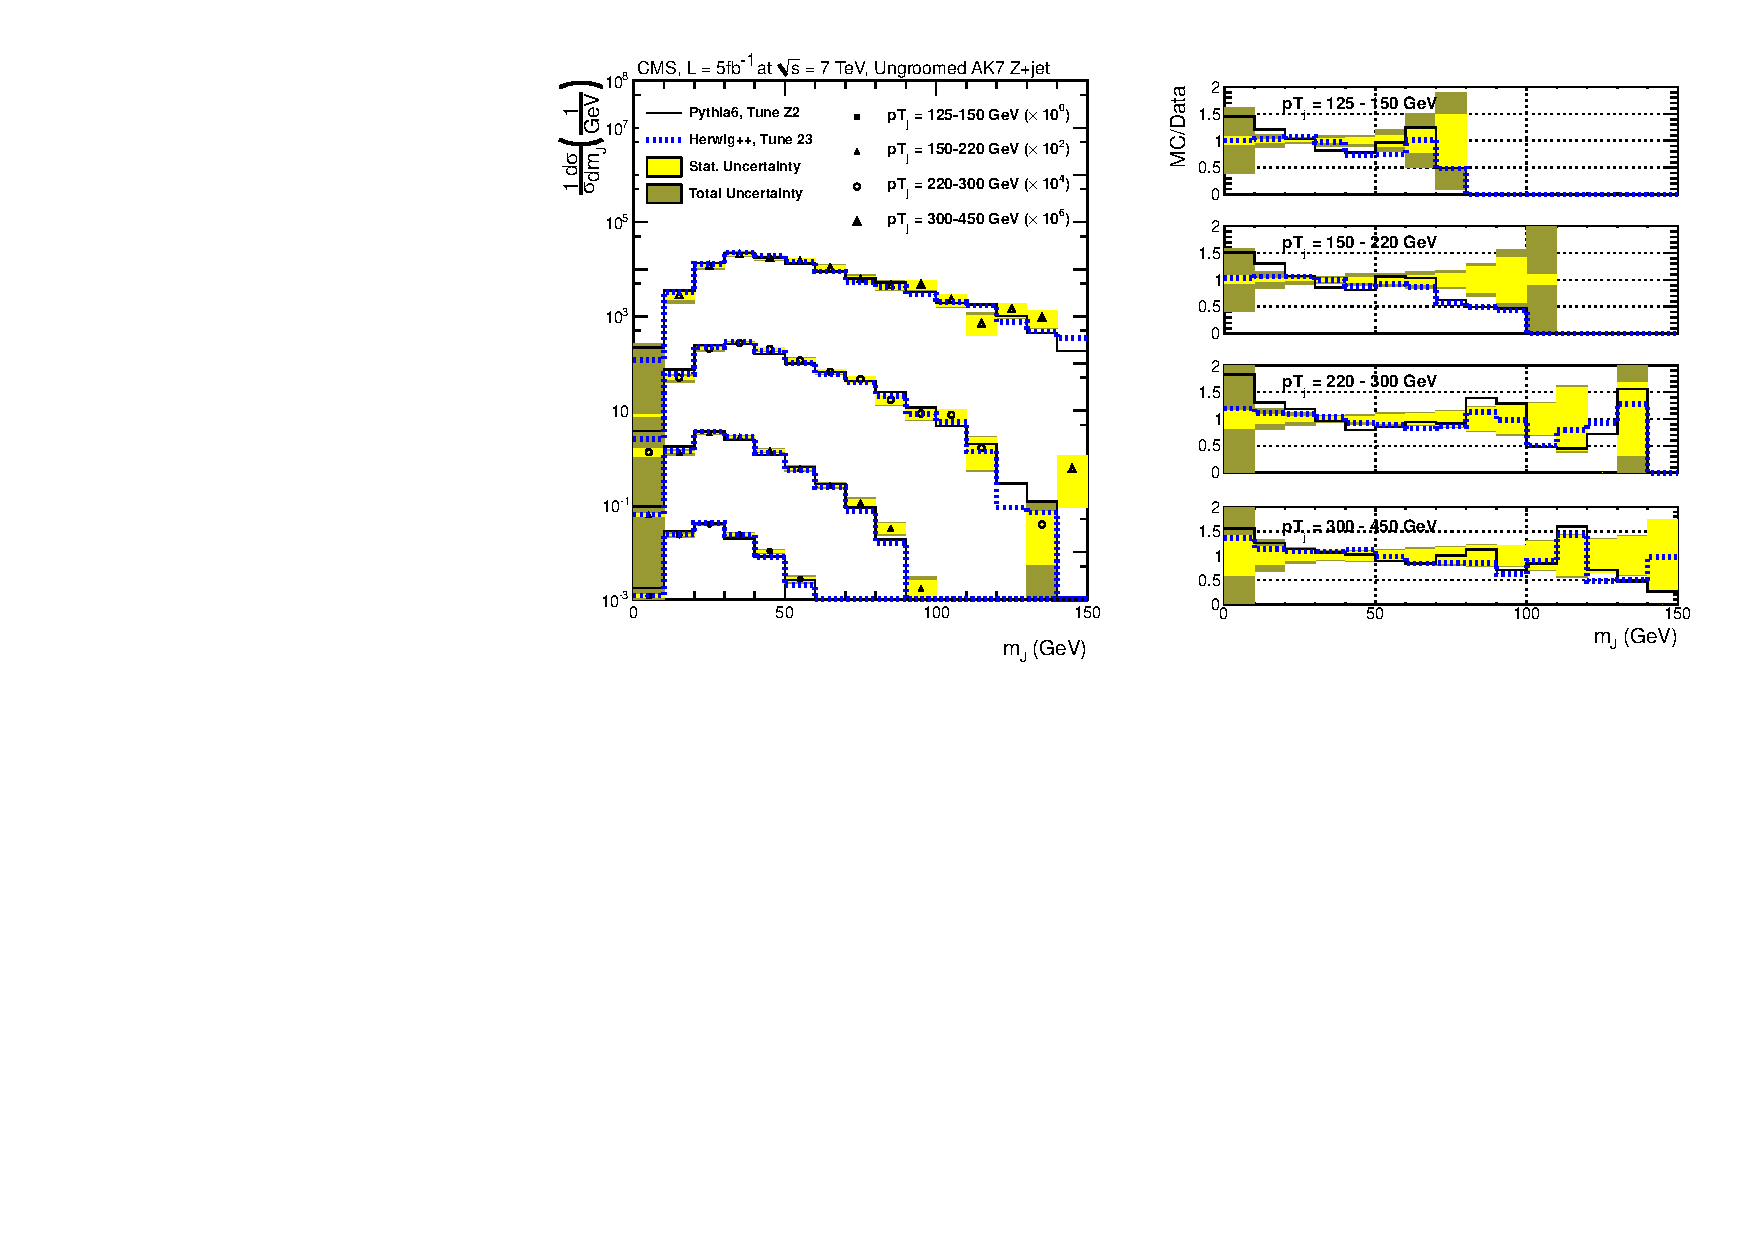
\includegraphics[width=0.99\textwidth]{figs/Zll/jetmassunf_ak7_log_Z.pdf}
\caption{Unfolded, ungroomed AK7 $m_J$ distribution for $\Z(\ell\ell)$+jet events. The data (black symbols) are compared to MC expectations from {\MADGRAPH}+\PYTHIA (solid lines) and \HERWIG (dotted lines) on the left. The ratio of MC to data is given on the right.
The statistical uncertainty is shown in light shading, and the total uncertainty in dark shading.}
\label{figs:AK7ZmmInt1}
\end{figure}

\begin{figure}[!htb]
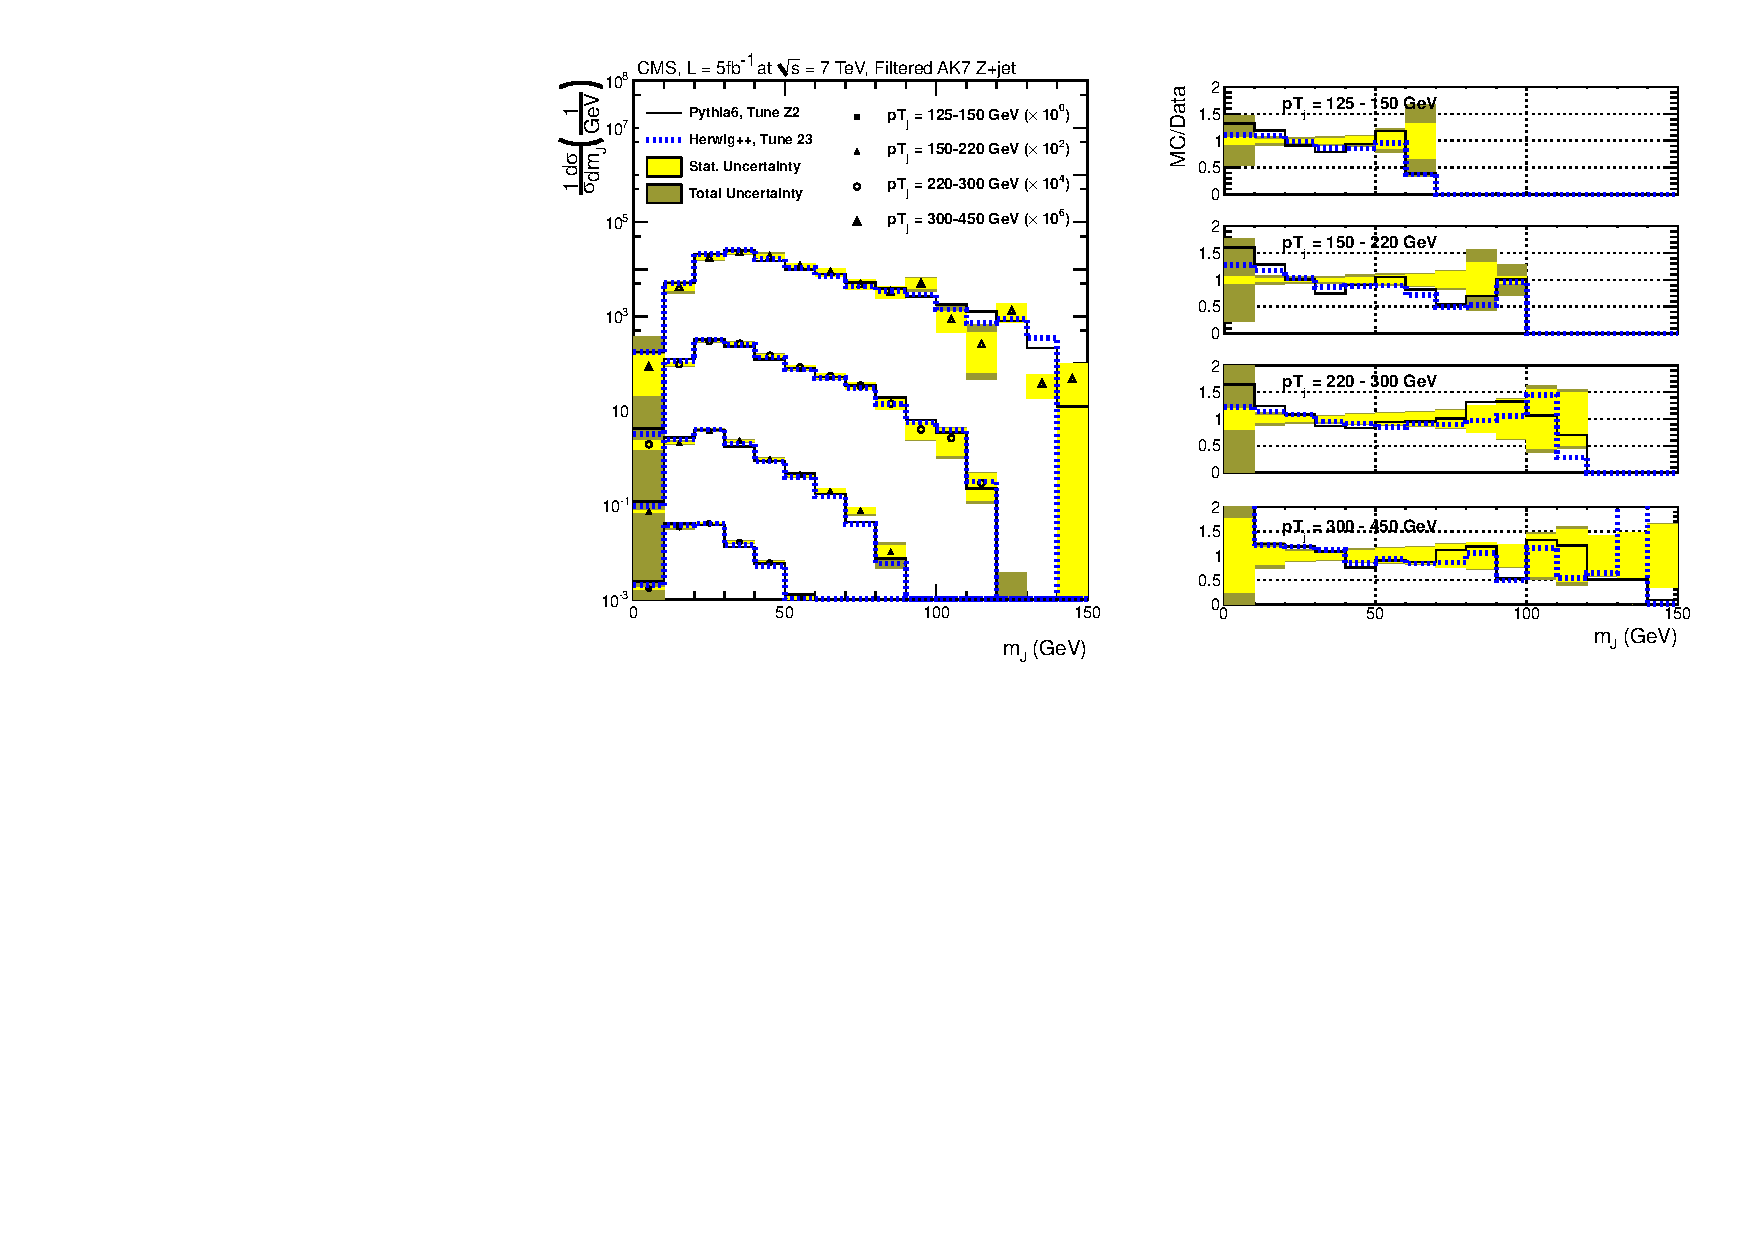
\includegraphics[width=0.99\textwidth]{figs/Zll/jetmassunf_ak7ft_log_Z.pdf}
\caption{Unfolded AK7 filtered $m_J$ distribution for $\Z(\ell\ell)$+jet events. The data (black symbols) are compared to MC expectations from {\MADGRAPH}+\PYTHIA (solid lines) and \HERWIG (dotted lines) on the left. The ratio of MC to data is given on the right.
The statistical uncertainty is shown in light shading, and the total uncertainty in dark shading.}
\label{figs:AK7ZmmInt3}
\end{figure}

\begin{figure}[!htb]
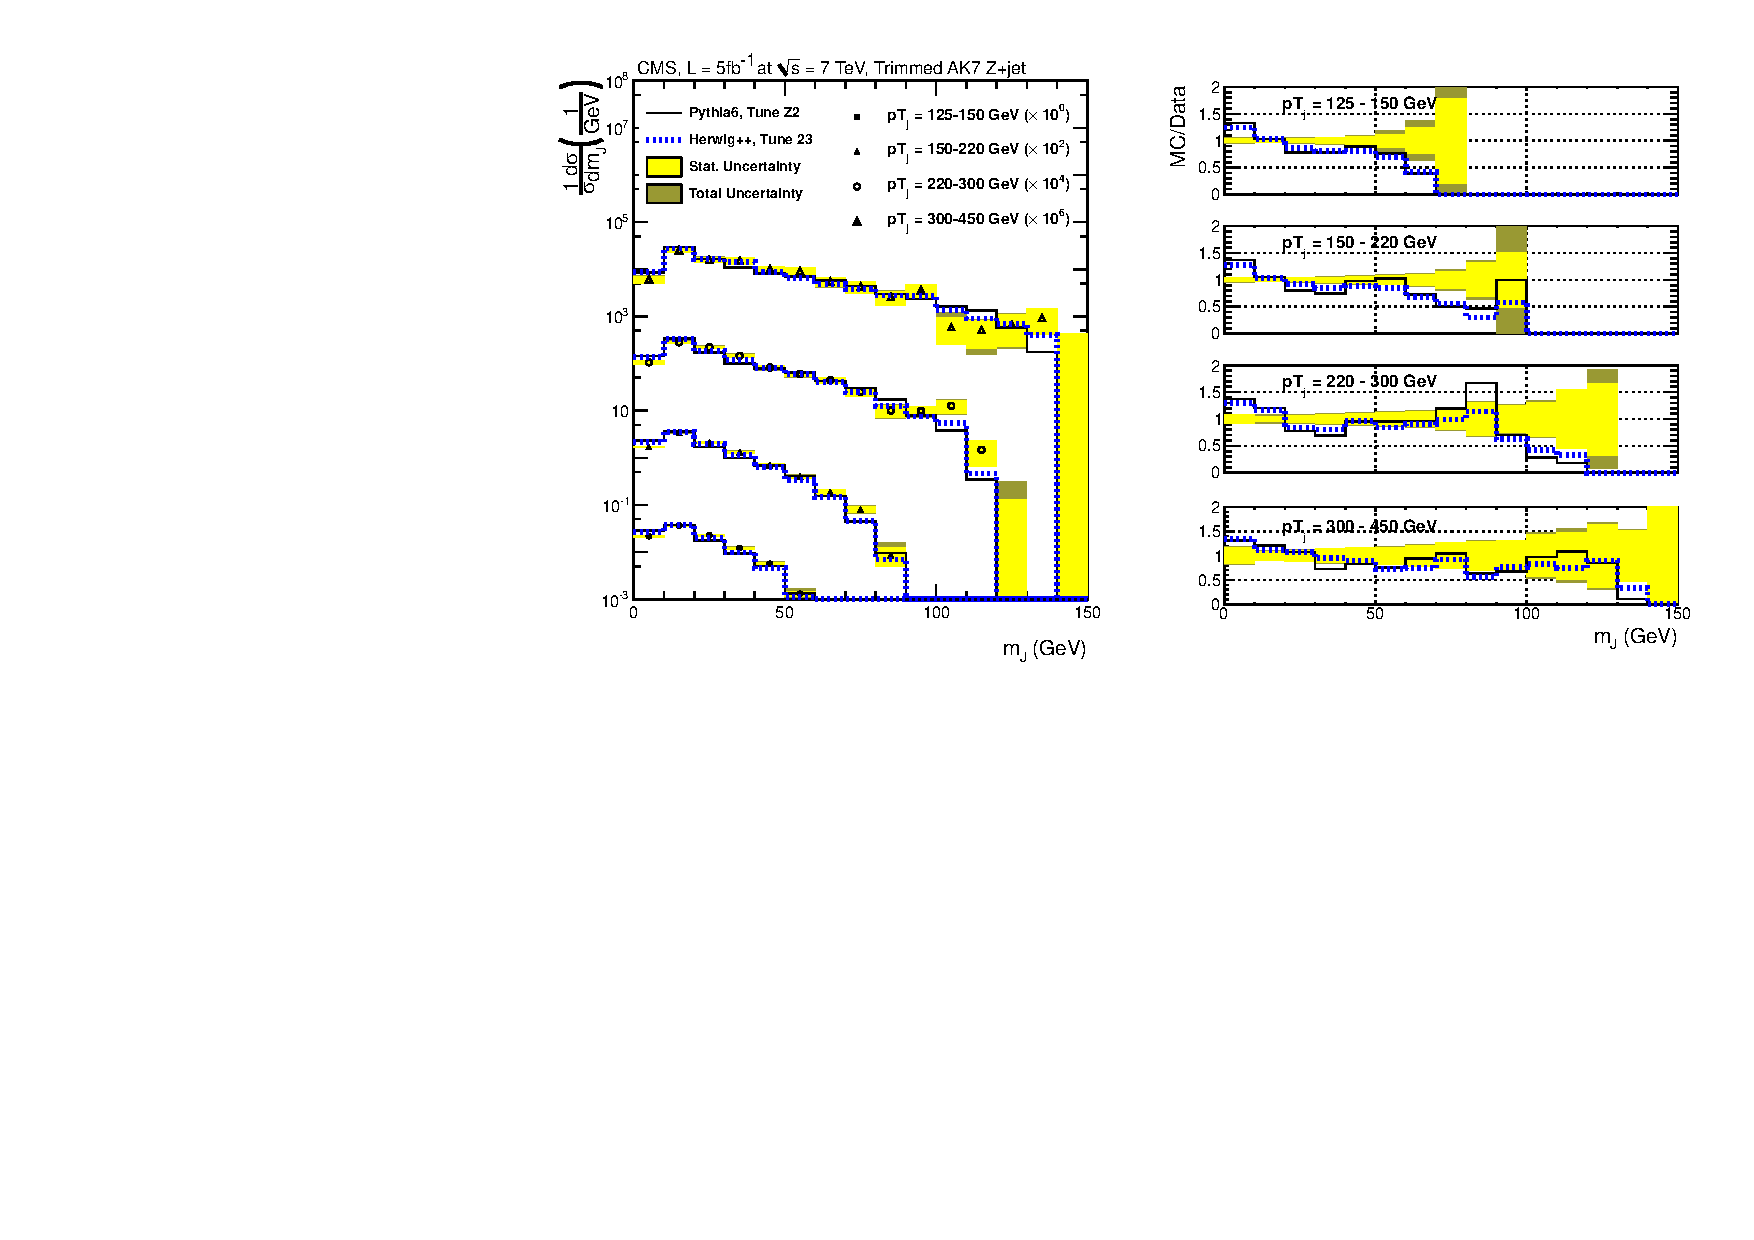
\includegraphics[width=0.99\textwidth]{figs/Zll/jetmassunf_ak7tr_log_Z.pdf}
\caption{Unfolded AK7 trimmed $m_J$ distribution for $\Z(\ell\ell)$+jet events. The data (black symbols) are compared to MC expectations from {\MADGRAPH}+\PYTHIA (solid lines) and \HERWIG (dotted lines) on the left. The ratio of MC to data is given on the right.
The statistical uncertainty is shown in light shading, and the total uncertainty in dark shading.}
\label{figs:AK7ZmmInt4}
\end{figure}

\begin{figure}[!htb]
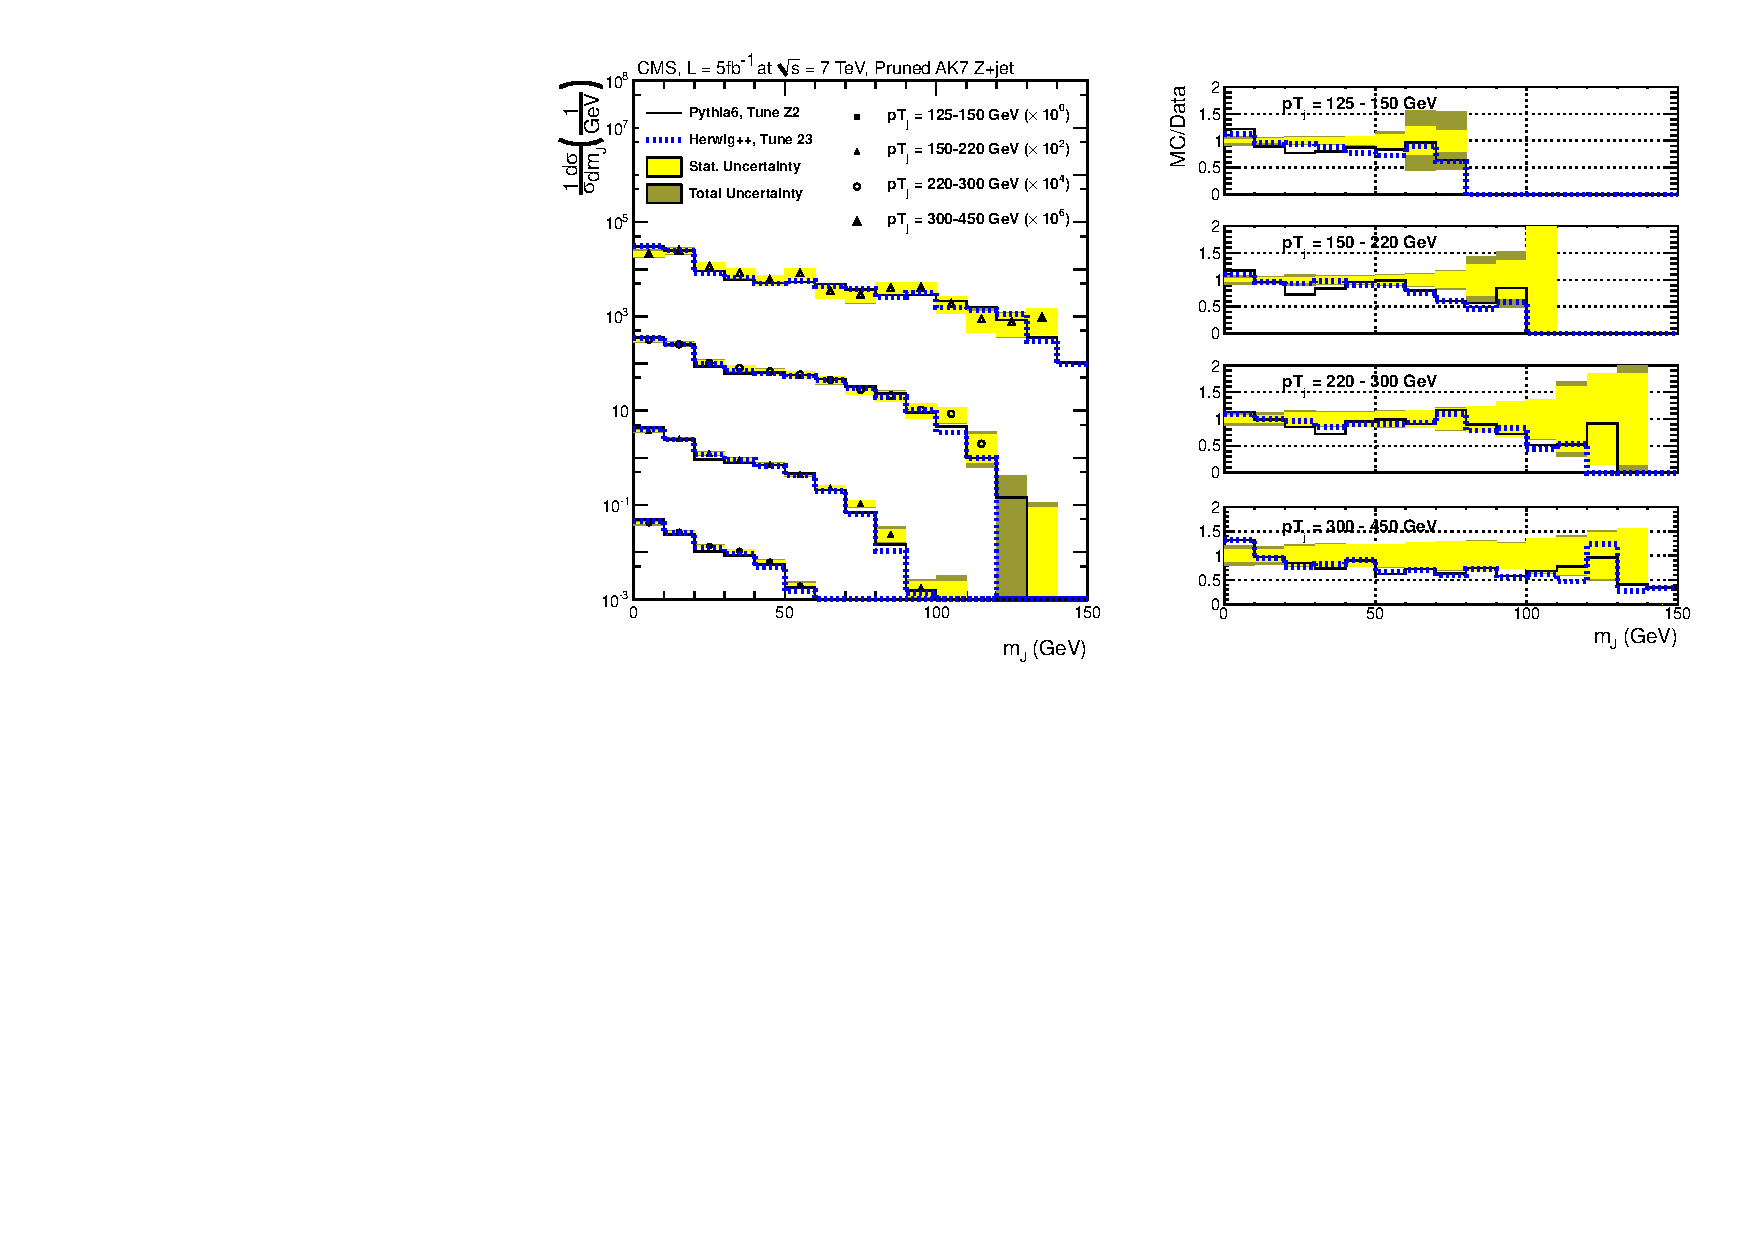
\includegraphics[width=0.99\textwidth]{figs/Zll/jetmassunf_ak7pr_log_Z.pdf}
\caption{Unfolded AK7 pruned $m_J$ distribution for $\Z(\ell\ell)$+jet events. The data (black symbols) are compared to MC expectations from {\MADGRAPH}+\PYTHIA (solid lines) and \HERWIG (dotted lines) on the left. The ratio of MC to data is given on the right.
The statistical uncertainty is shown in light shading, and the total uncertainty in dark shading.}
\label{figs:AK7ZmmInt2}
\end{figure}

\begin{figure}[!htb]
\centering
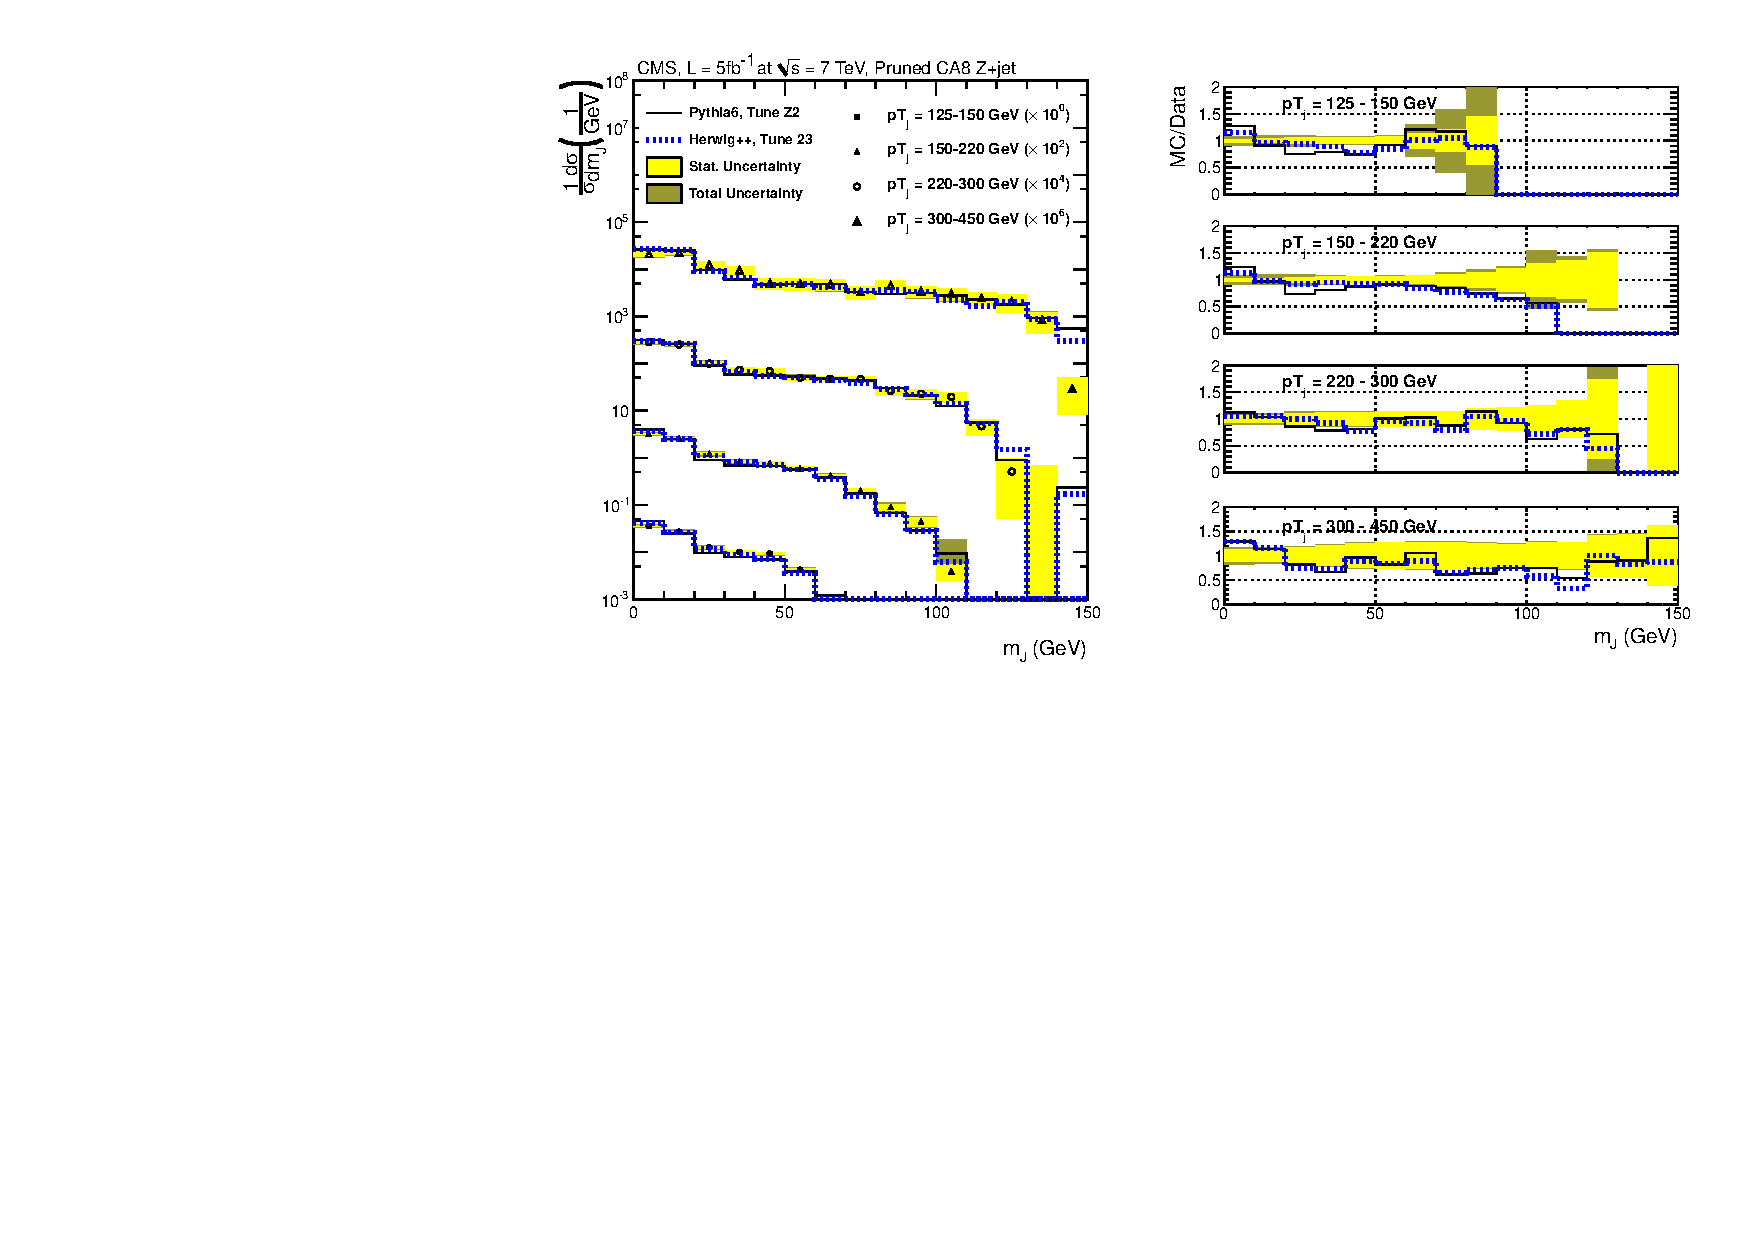
\includegraphics[width=0.99\textwidth]{figs/Zll/jetmassunf_ca8pr_log_Z.pdf}
\caption{Unfolded CA8 pruned $m_J$ distribution for $\Z(\ell\ell)$+jet events. The data (black symbols) are compared to MC expectations from {\MADGRAPH}+\PYTHIA (solid lines) and \HERWIG (dotted lines) on the left. The ratio of MC to data is given on the right.
The statistical uncertainty is shown in light shading, and the total uncertainty in dark shading.}
\label{figs:prunedZmmInt1}
\end{figure}

\begin{figure}[!htb]
\centering
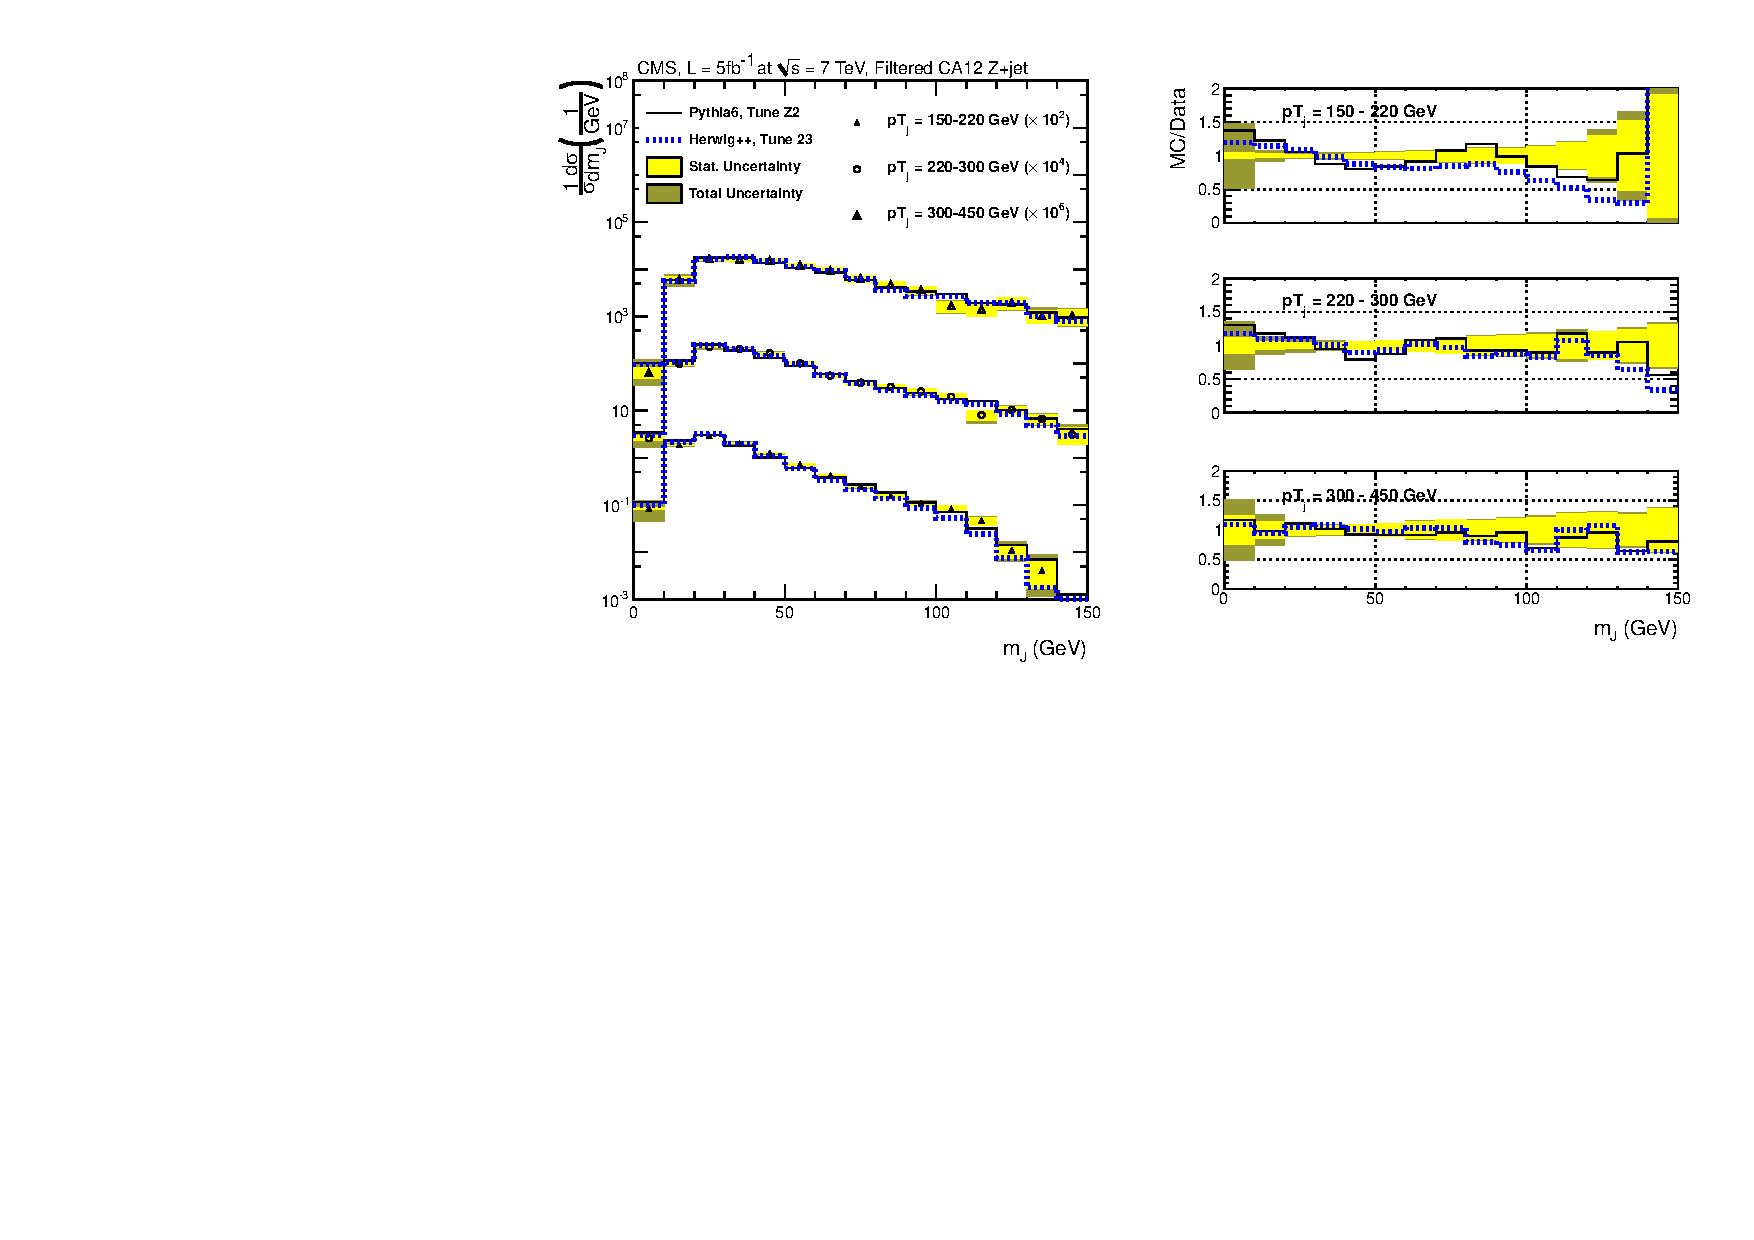
\includegraphics[width=0.99\textwidth]{figs/Zll/jetmassunf_ca12ft_log_Z.pdf}
\caption{Unfolded CA12 filtered $m_J$ distribution for $\Z(\ell\ell)$+jet events. The data (black symbols) are compared to MC expectations from {\MADGRAPH}+\PYTHIA (solid lines) and \HERWIG (dotted lines) on the left. The ratio of MC to data is given on the right.
The statistical uncertainty is shown in light shading, and the total uncertainty in dark shading.}
\label{figs:prunedZmmInt2}
\end{figure}


\clearpage


%\subsection{W$(\ell\nu)$ +jet Analysis}

%Fig.~\ref{figs:AK7WmnInt1}-\ref{figs:AK7WmnInt4} shows the $m_J$ distribution for AK7 jets in W$(\ell\nu)$ +jet events, for the different clustering algorithm studied: ungroomed, pruned, trimmed, and filtered respectively.
%Fig.~\ref{figs:prunedWmnInt1}-\ref{figs:prunedWmnInt2} shows the $m_J$ distribution for pruned CA8 and filtered CA12 jets in W$(\ell\nu)$ +jet events.
%The simulation has a good agreement with data: similar observations as the ones reported for the Z+jet events apply also here.

\begin{figure}[!htb]
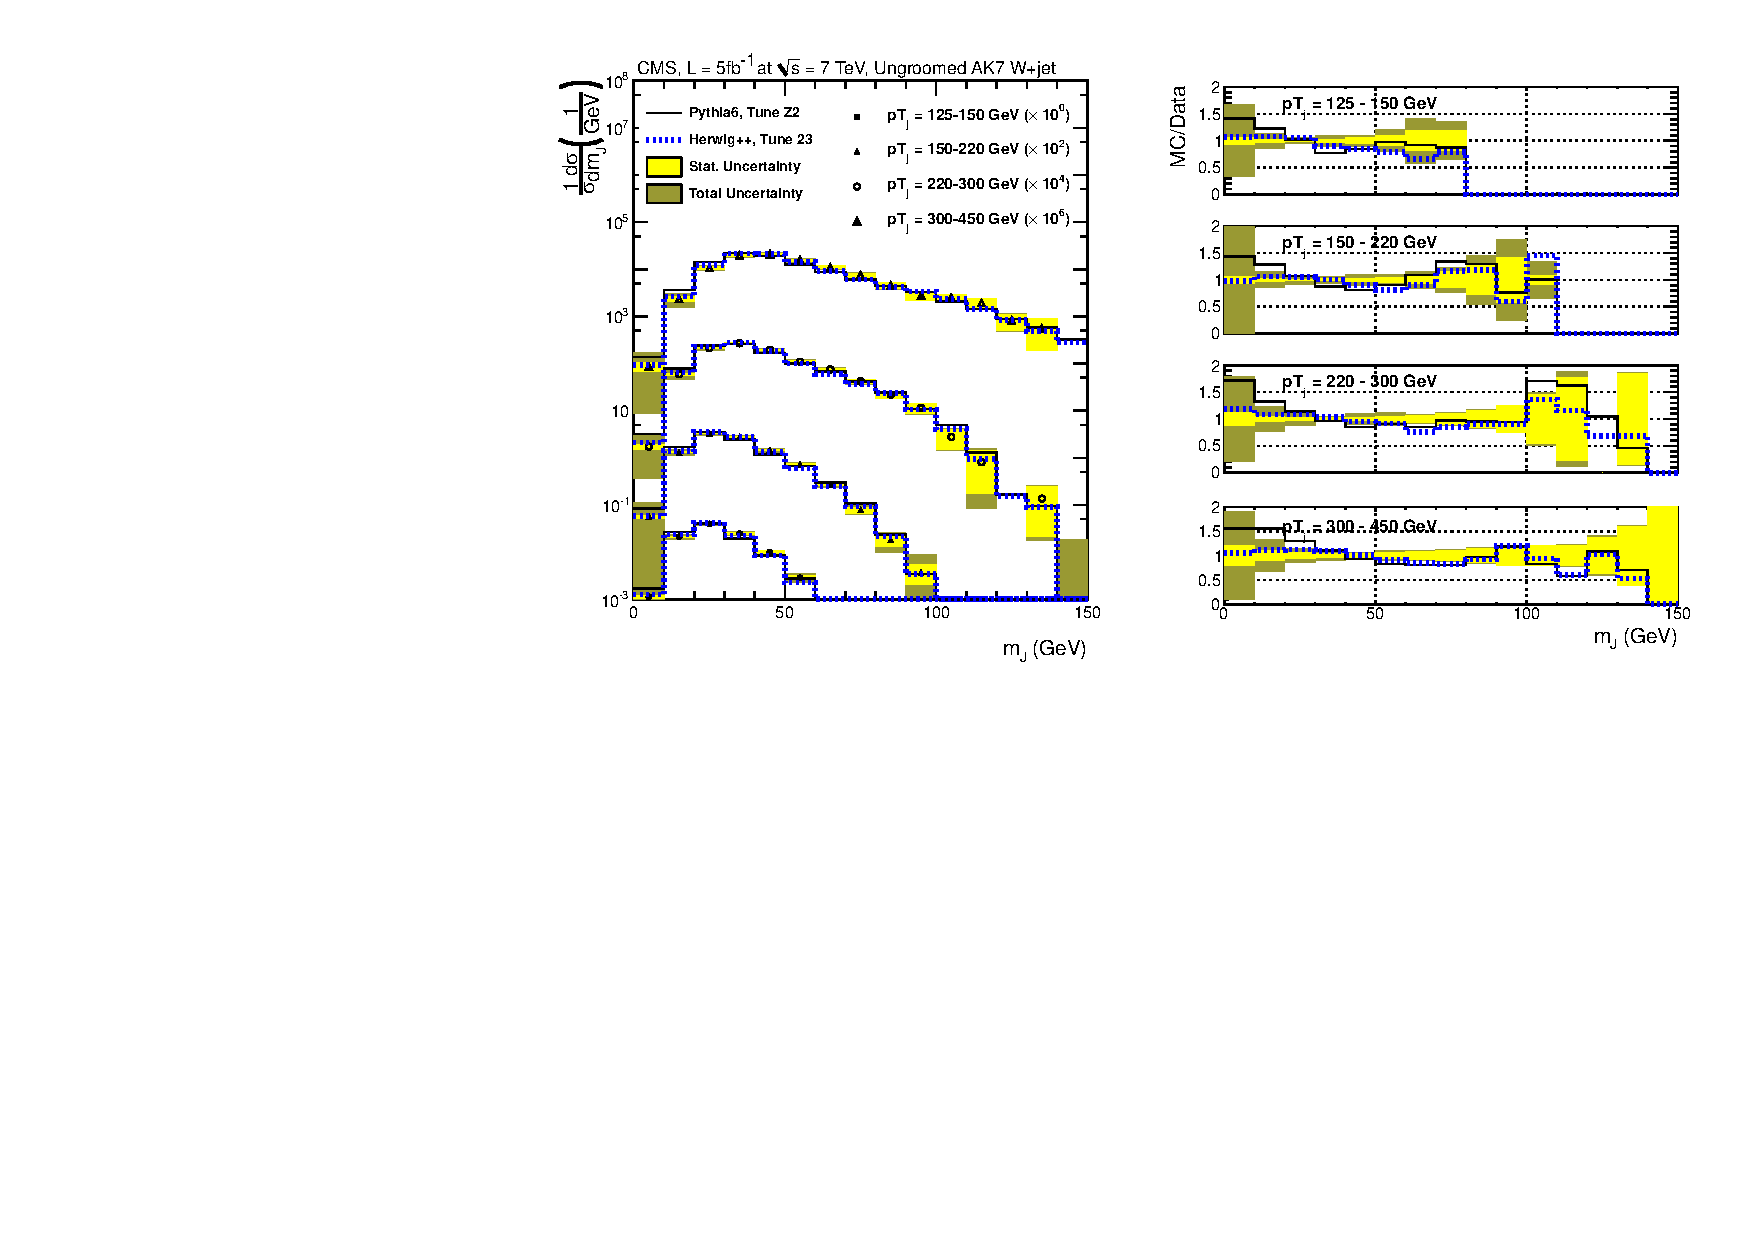
\includegraphics[width=0.99\textwidth]{figs/Wln/jetmassunf_ak7_log_W.pdf}
\caption{Distributions in $m_J$ for unfolded, ungroomed AK7 jets in  \PW$(\ell\nu_\ell)$+jet events. The data (black symbols) are compared to MC expectations from {\MADGRAPH}+\PYTHIA (solid lines) and \HERWIG (dotted lines) on the left. The ratios of MC to data are given on the right.
The statistical uncertainty is shown in light shading, and the total uncertainty in dark shading.}
\label{figs:AK7WmnInt1}
\end{figure}

\begin{figure}[!htb]
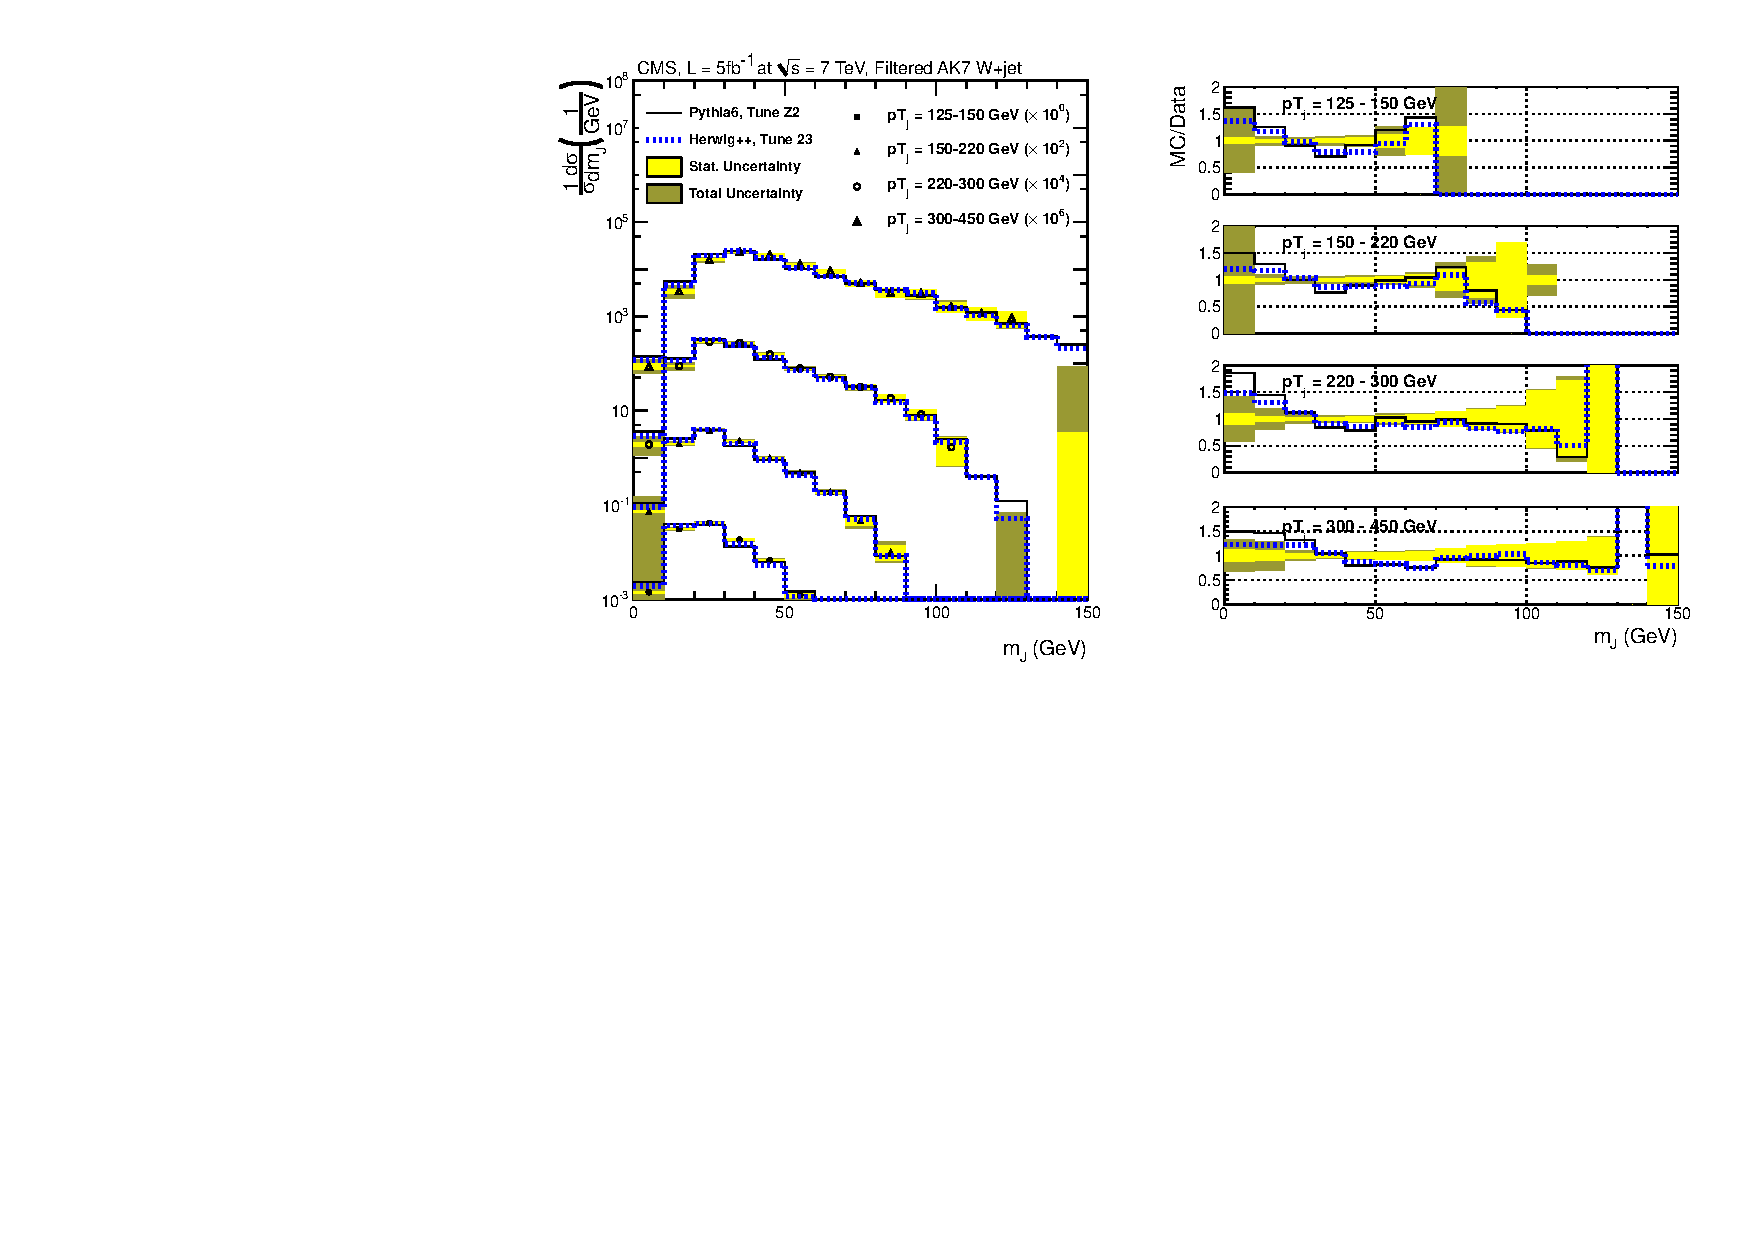
\includegraphics[width=0.99\textwidth]{figs/Wln/jetmassunf_ak7ft_log_W.pdf}
\caption{Distributions in $m_J$ for unfolded, filtered AK7 jets in \PW$(\ell\nu_\ell)$+jet events. The data (black symbols) for different bins in $\pt$ are compared to MC expectations from {\MADGRAPH}+\PYTHIA (solid lines) and \HERWIG (dotted lines) on the left. The ratios of MC to data are given on the right.
The statistical uncertainty is shown in light shading, and the total uncertainty in dark shading.}
\label{figs:AK7WmnInt3}
\end{figure}

\begin{figure}[!htb]
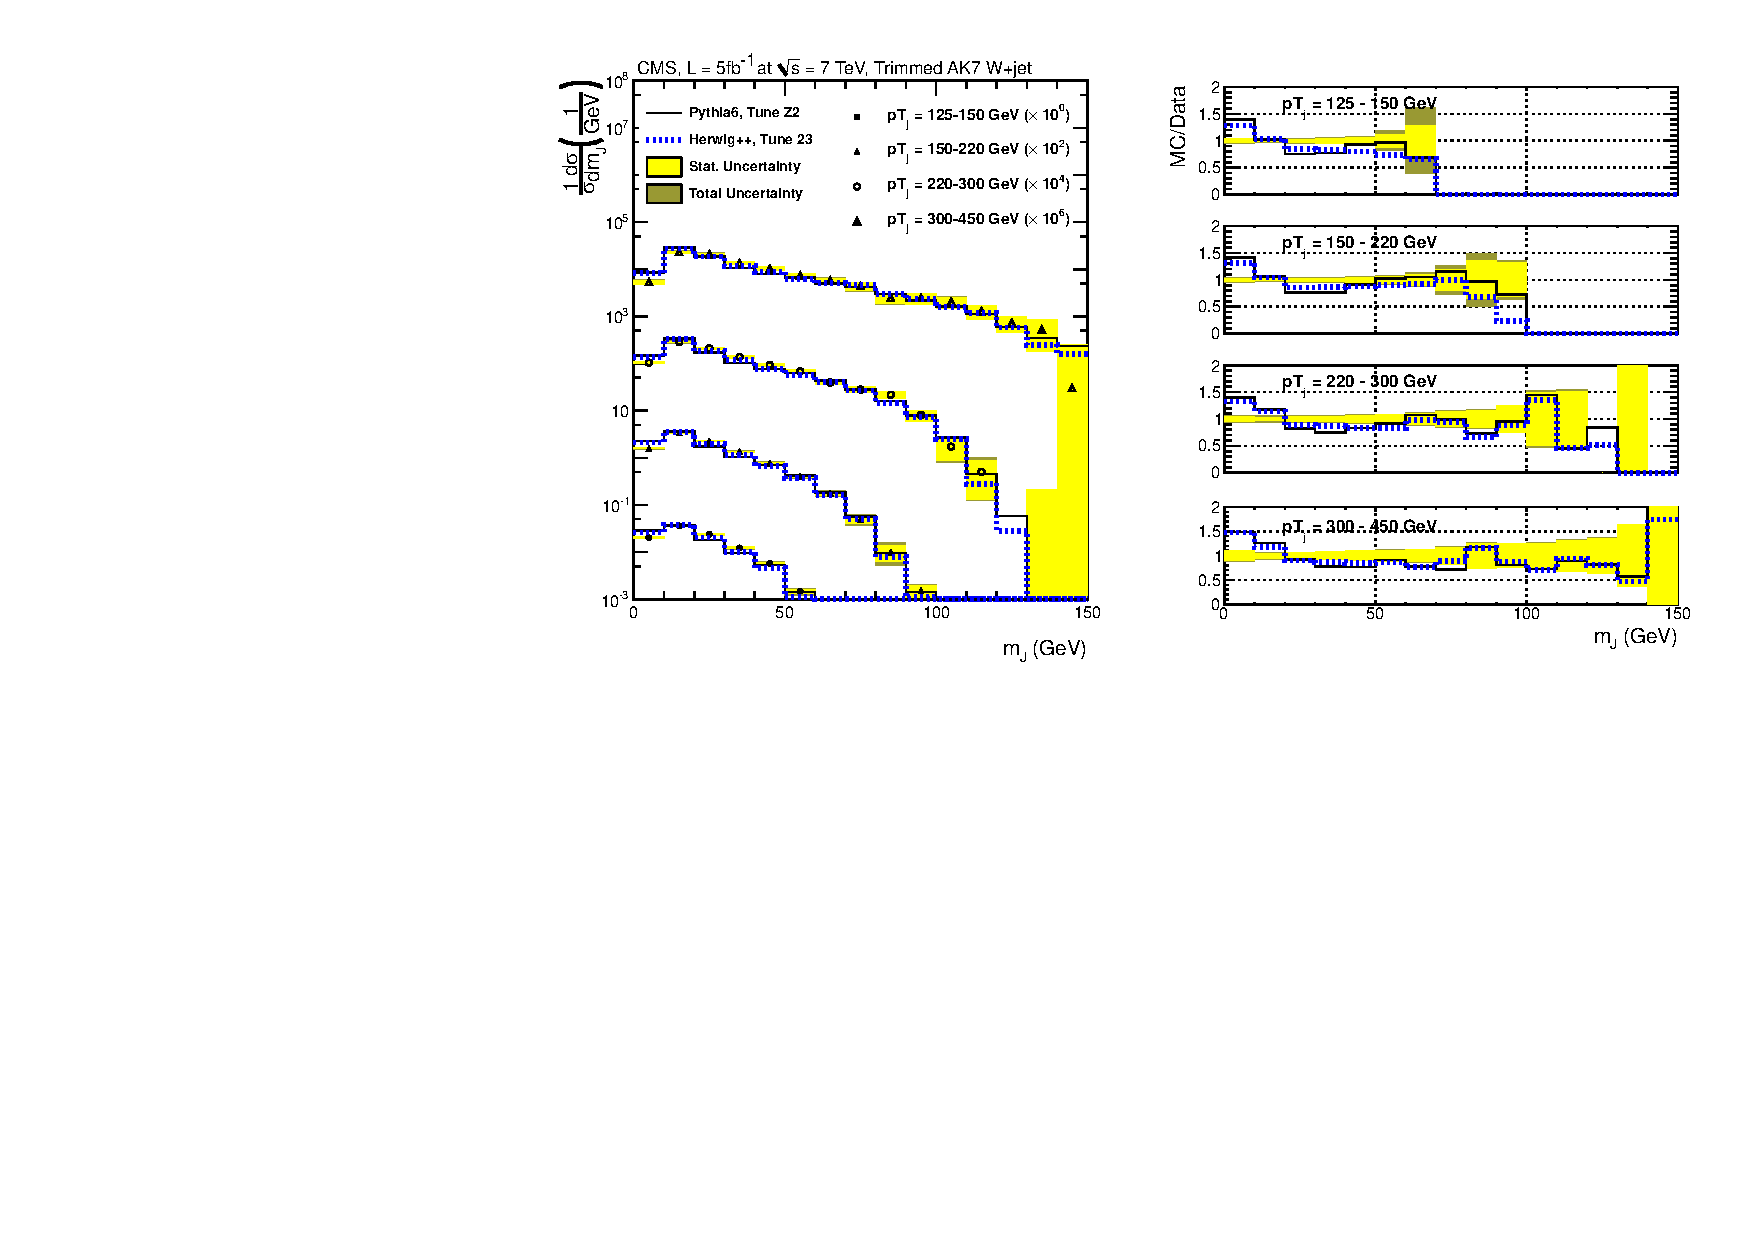
\includegraphics[width=0.99\textwidth]{figs/Wln/jetmassunf_ak7tr_log_W.pdf}
\caption{Distributions in $m_J$ for unfolded, trimmed AK7 jets in \PW$(\ell\nu_\ell)$+jet events. The data (black symbols) for different bins in $\pt$ are compared to MC expectations from {\MADGRAPH}+\PYTHIA (solid lines) and \HERWIG (dotted lines) on the left. The ratios of MC to data are given on the right.
The statistical uncertainty is shown in light shading, and the total uncertainty in dark shading.}
\label{figs:AK7WmnInt4}
\end{figure}

\begin{figure}[!htb]
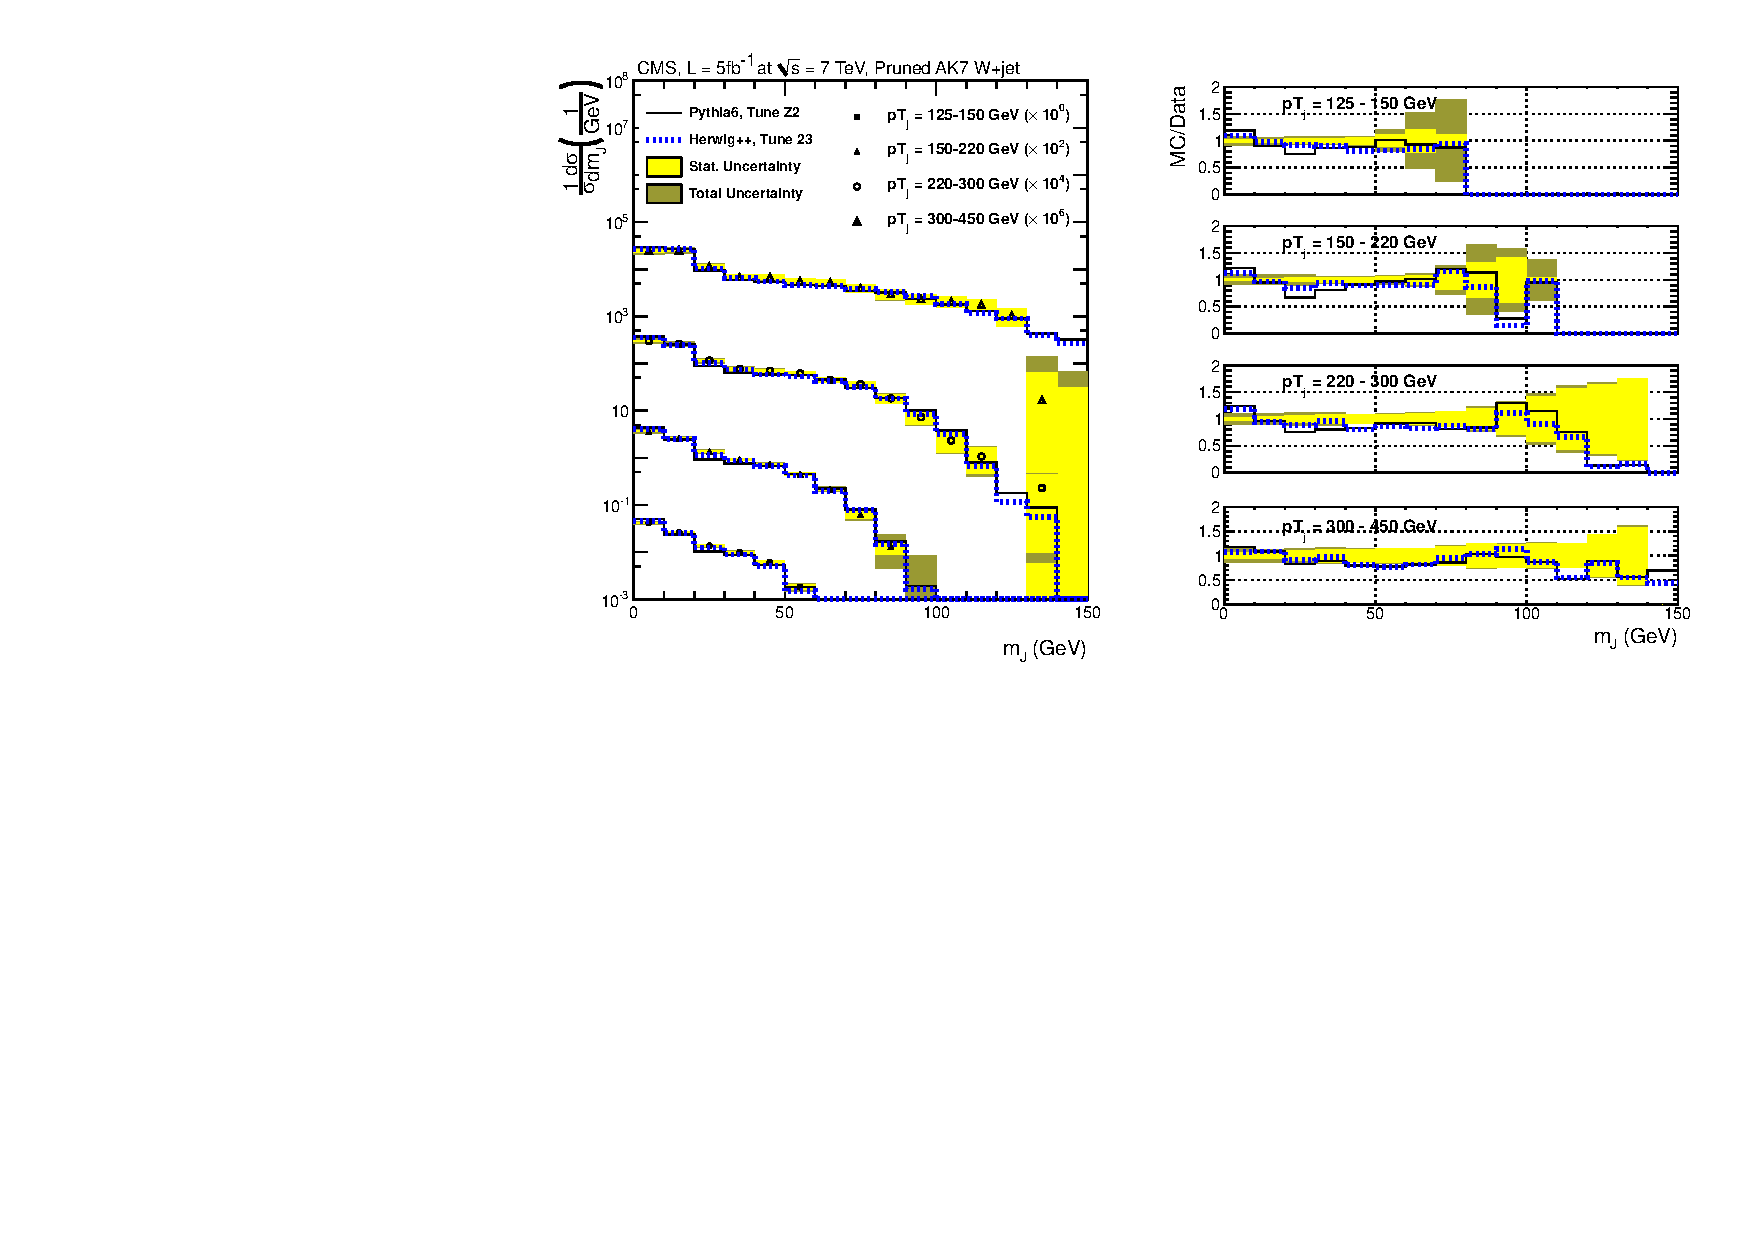
\includegraphics[width=0.99\textwidth]{figs/Wln/jetmassunf_ak7pr_log_W.pdf}
\caption{Distributions in $m_J$ for unfolded, pruned AK7 jets in \PW$(\ell\nu_\ell)$+jet events. The data (black symbols) for different bins in $\pt$ are compared to MC expectations from {\MADGRAPH}+\PYTHIA (solid lines) and \HERWIG (dotted lines) on the left. The ratios of MC to data are given on the right.
The statistical uncertainty is shown in light shading, and the total uncertainty in dark shading.}
\label{figs:AK7WmnInt2}
\end{figure}

\begin{figure}[!htb]
\centering
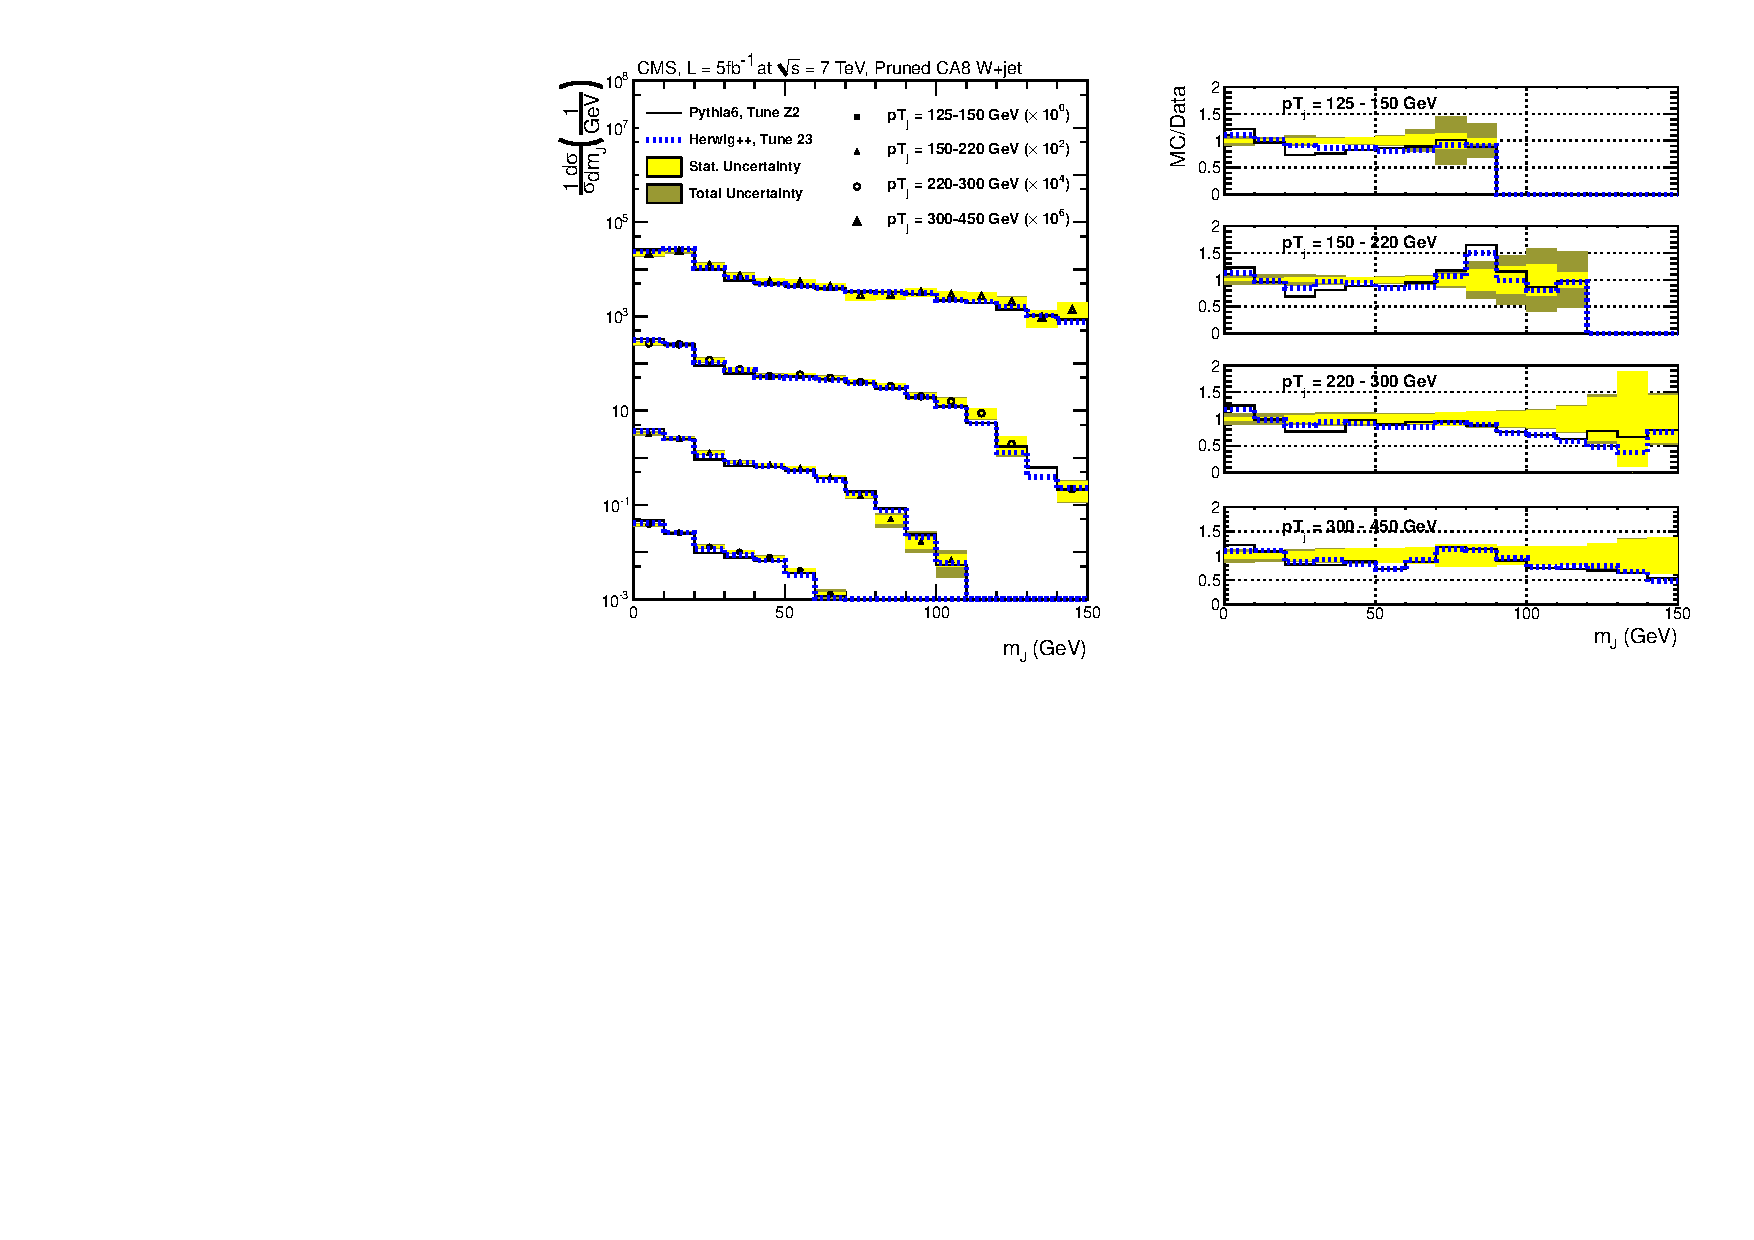
\includegraphics[width=0.99\textwidth]{figs/Wln/jetmassunf_ca8pr_log_W.pdf}
\caption{Distributions in $m_J$ for unfolded, pruned CA8 jets in \PW$(\ell\nu_\ell)$+jet events. The data (black symbols) for different bins in $\pt$ are compared to MC expectations from {\MADGRAPH}+\PYTHIA (solid lines) and \HERWIG (dotted lines) on the left. The ratios of MC to data are given on the right.
The statistical uncertainty is shown in light shading, and the total uncertainty in dark shading.}
\label{figs:prunedWmnInt1}
\end{figure}

\begin{figure}[!htb]
\centering
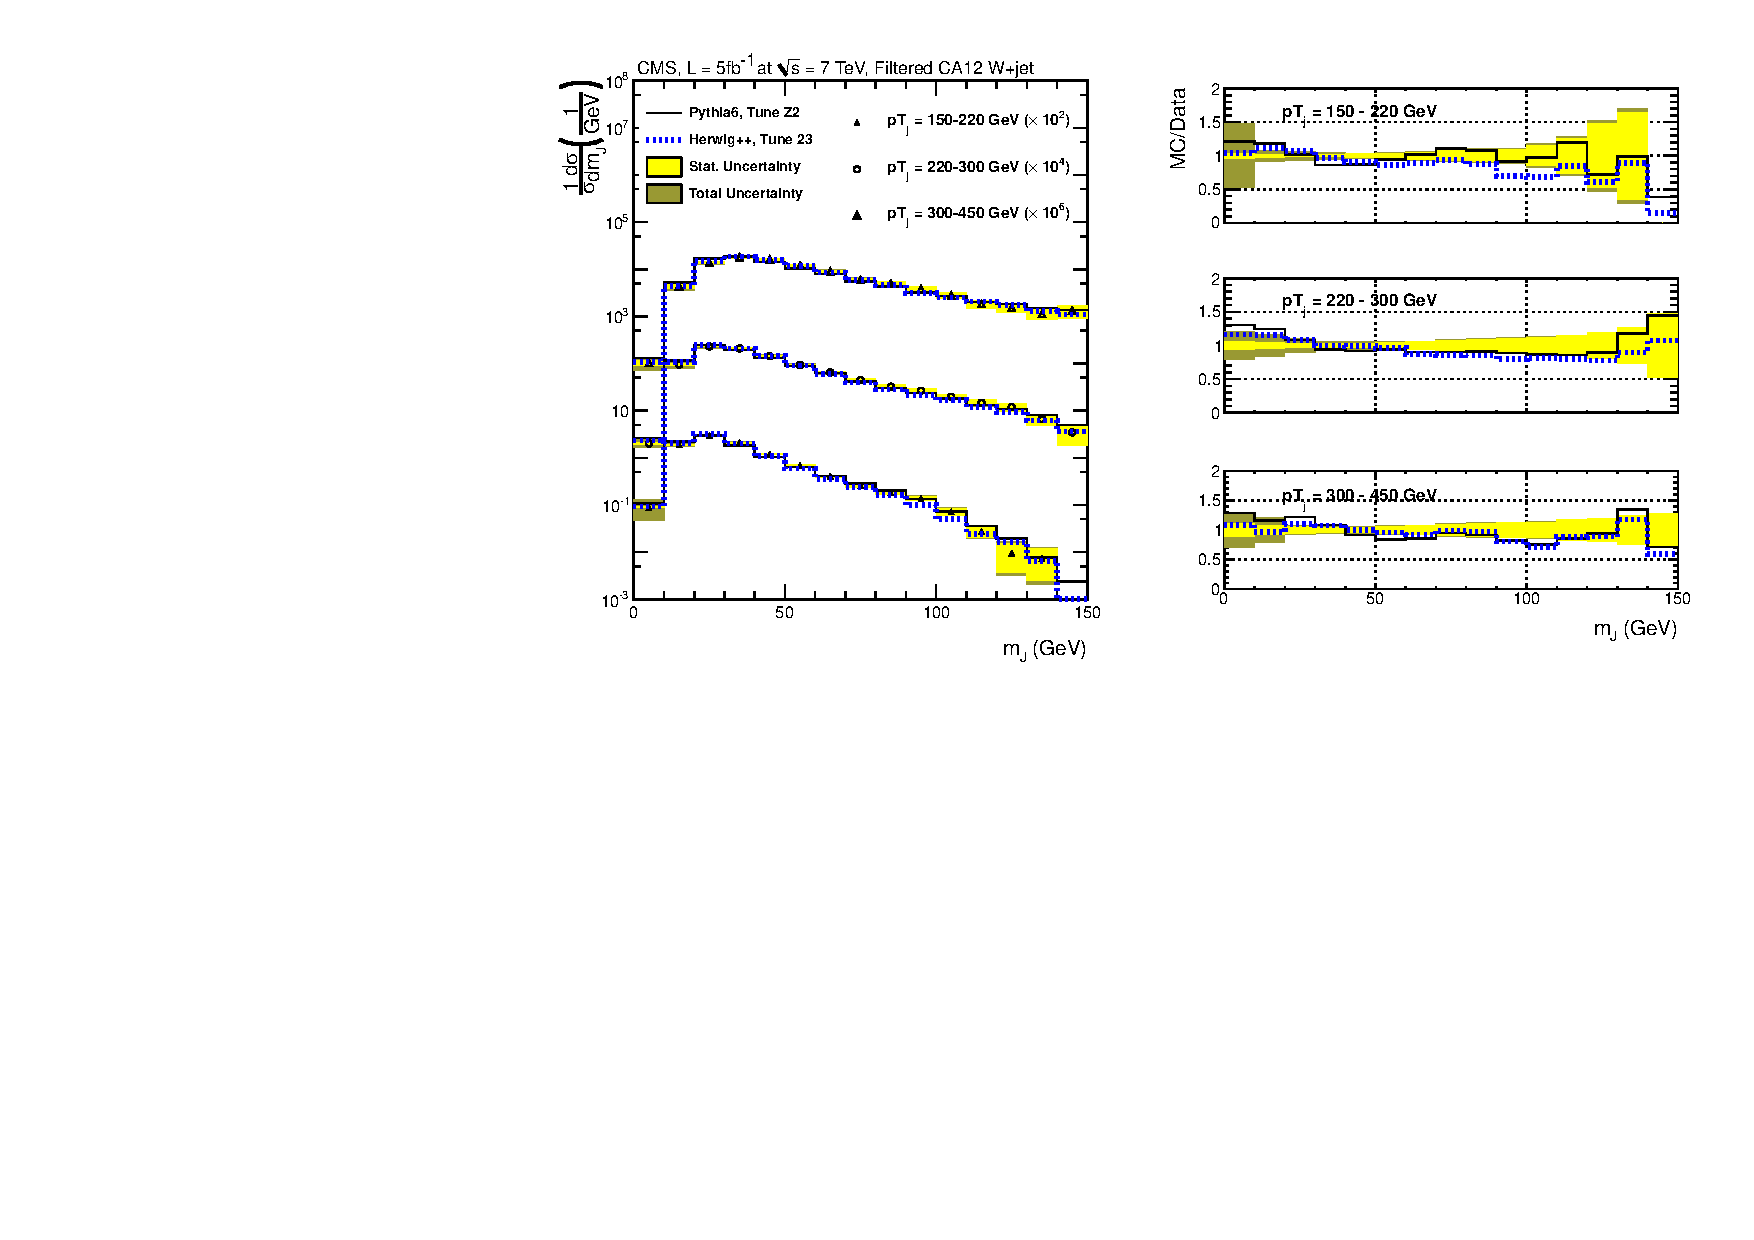
\includegraphics[width=0.99\textwidth]{figs/Wln/jetmassunf_ca12ft_log_W.pdf}
\caption{Distributions in $m_J$ for unfolded, filtered CA12 jets in \PW$(\ell\nu_\ell)$+jet events. The data (black symbols) for different bins in $\pt$ are compared to MC expectations from {\MADGRAPH}+\PYTHIA (solid lines) and \HERWIG (dotted lines) on the left. The ratios of MC to data are given on the right.
The statistical uncertainty is shown in light shading, and the total uncertainty in dark shading.}
\label{figs:prunedWmnInt2}
\end{figure}

\clearpage






